% anhang.tex
\chapter{Visualisierung des Tomate Yellow Leaf Curl Virus}
\label{anahngc}
\begin{figure}[h!]
	\centering
	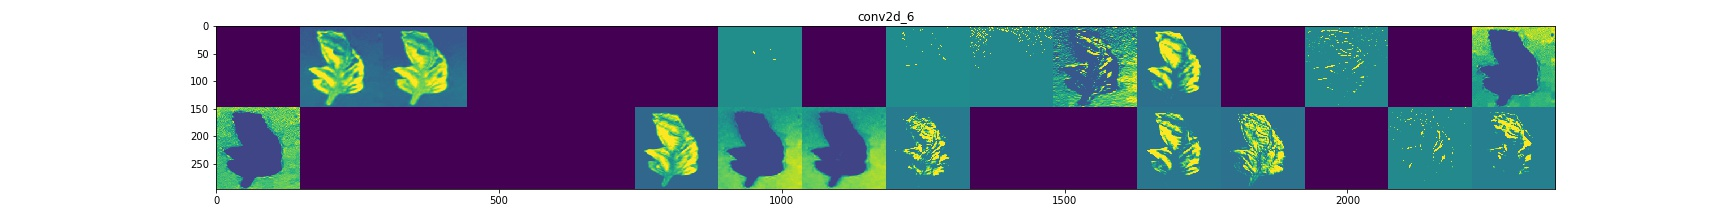
\includegraphics[width=\textwidth]{visualisierungen/yellow/activation/yellow0.JPG}
	\caption{Visualisierung der Aktivierungswerte in der ersten Faltungschicht von dem TYLCV-Virus (eigene Darstellung).}
	\label{}
\end{figure}

\begin{figure}[h!]
	\centering
	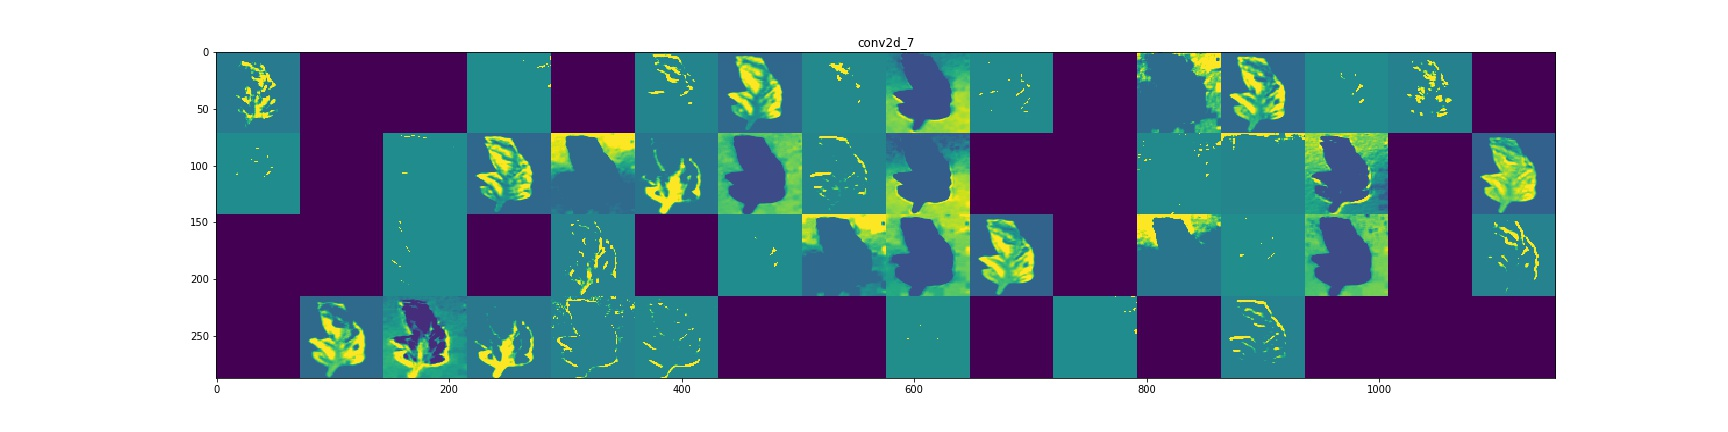
\includegraphics[width=\textwidth]{visualisierungen/yellow/activation/yellow3.JPG}
	\caption{Visualisierung der Aktivierungswerte in der zweiten Faltungschicht von dem TYLCV-Virus (eigene Darstellung).}
	\label{}
\end{figure}

\begin{figure}[h!]
	\centering
	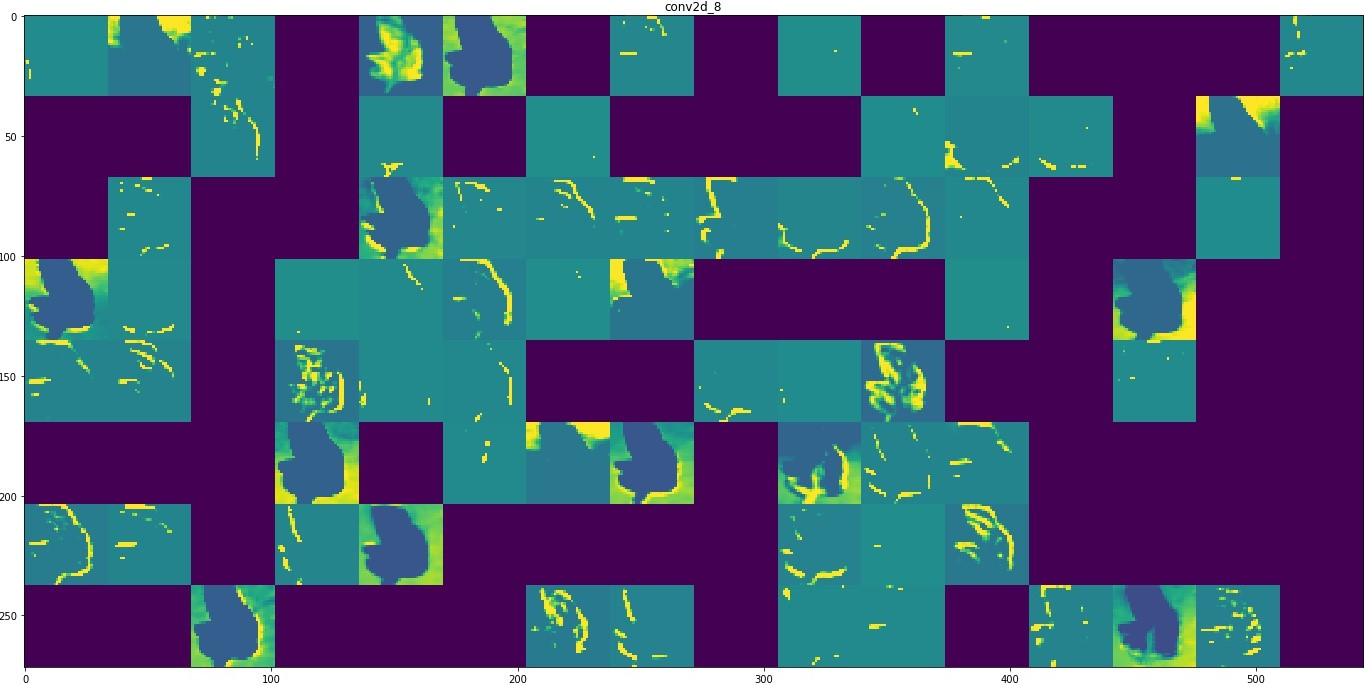
\includegraphics[width=\textwidth]{visualisierungen/yellow/activation/yellow6.JPG}
	\caption{Visualisierung der Aktivierungswerte in der dritten Faltungschicht von dem TYLCV-Virus (eigene Darstellung).}
	\label{}
\end{figure}

\begin{figure}[h!]
	\centering
	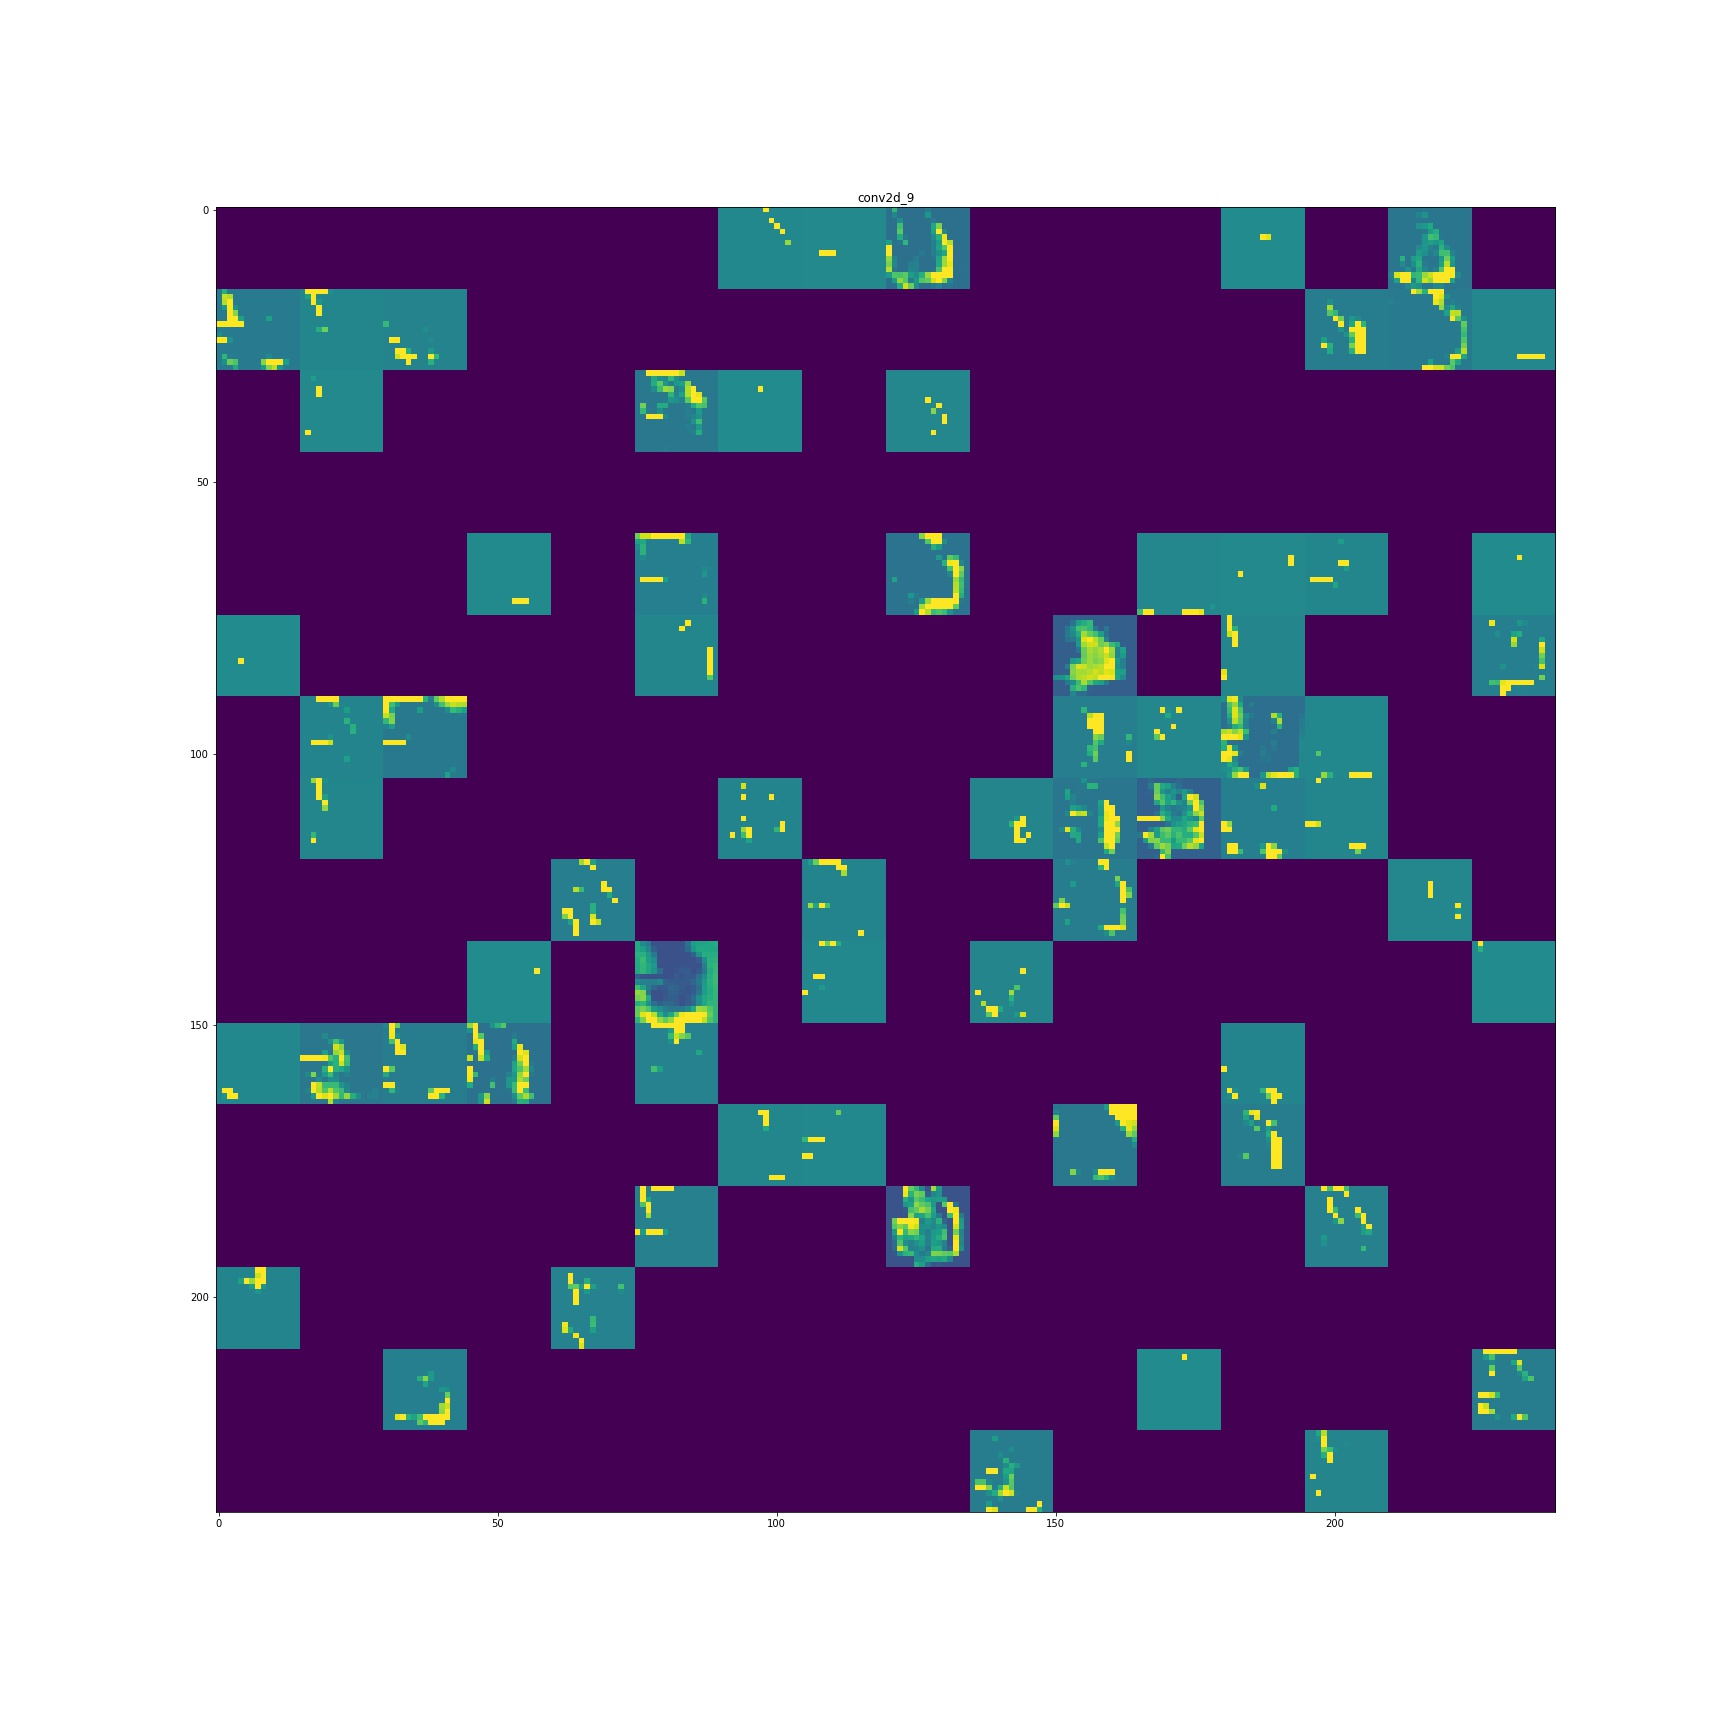
\includegraphics[width=\textwidth]{visualisierungen/yellow/activation/yellow8.JPG}
	\caption{Visualisierung der Aktivierungswerte in der vierten Faltungschicht von dem TYLCV-Virus (eigene Darstellung).}
	\label{yellow8_anhang}
\end{figure}

\begin{figure}[h!]
	\centering
	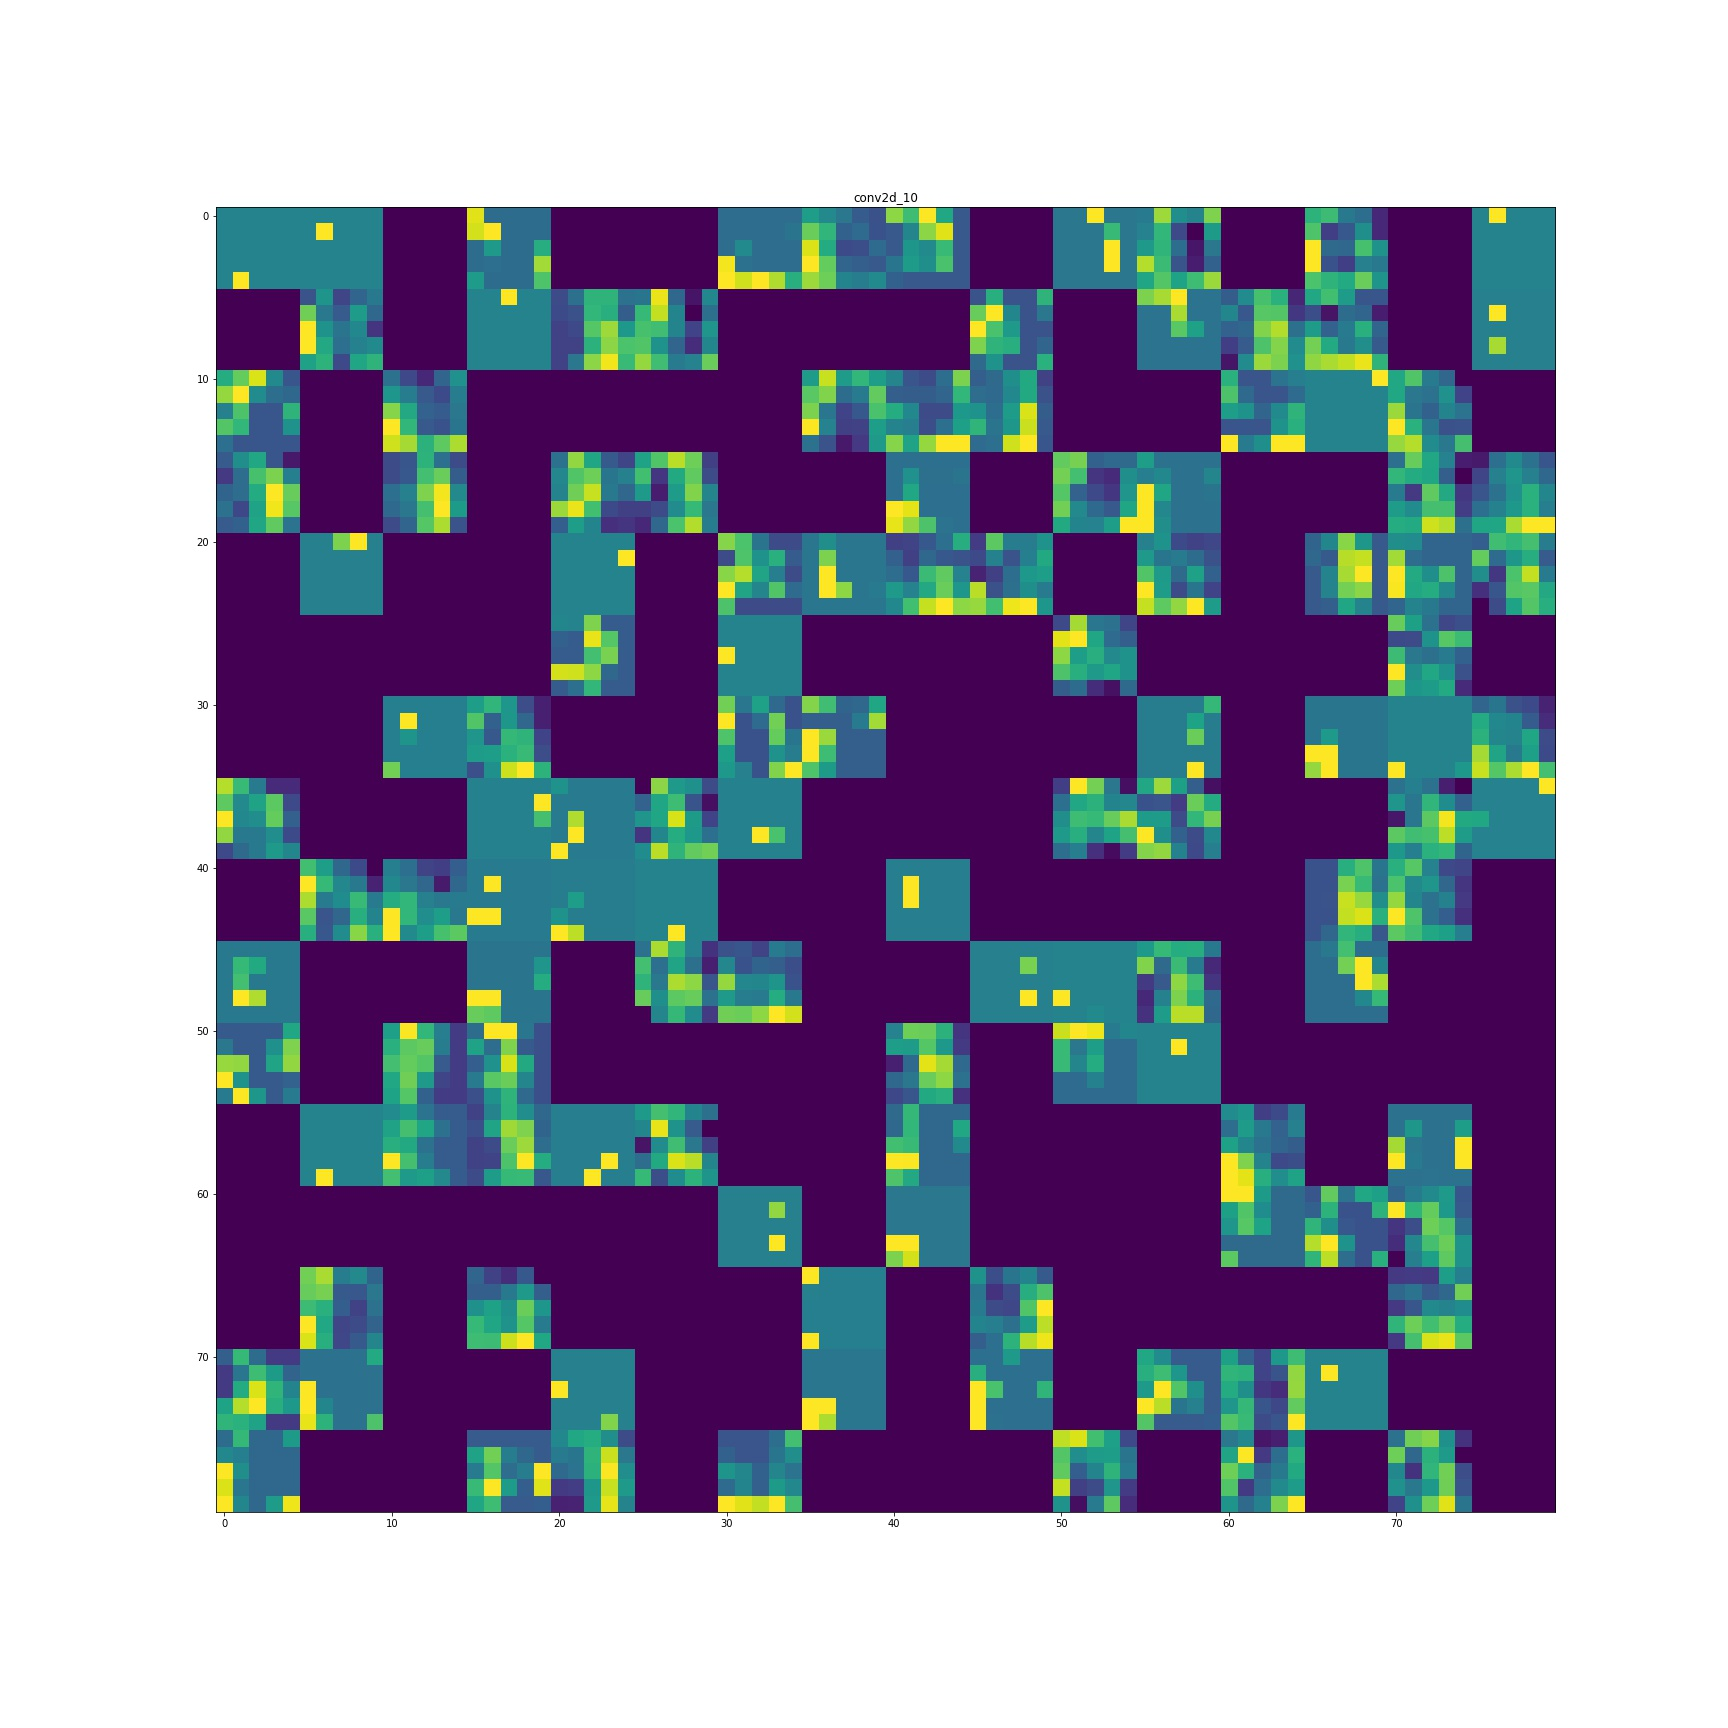
\includegraphics[width=\textwidth]{visualisierungen/yellow/activation/yellow10.JPG}
	\caption{Visualisierung der Aktivierungswerte in der fünften Faltungschicht von dem TYLCV-Virus (eigene Darstellung).}
	\label{}
\end{figure}

%%%%%%%%%%%%%%%%%%%%%%%%%%%%%%%%%%%%%%%%%%%%%%

\begin{figure}[h!]
	\centering
	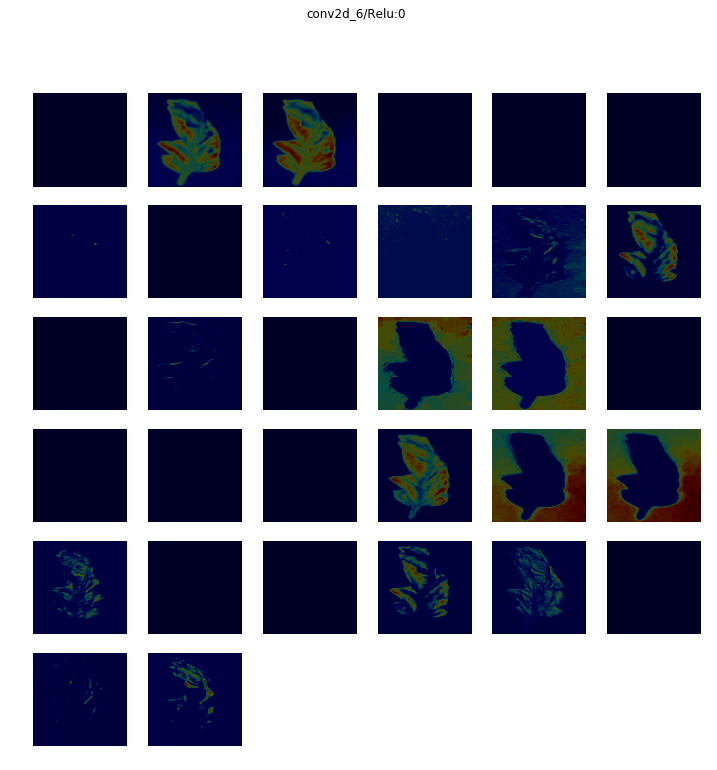
\includegraphics[width=\textwidth]{visualisierungen/yellow/heapmap_mit/conv2d_6.png}
	\caption{Visualisierung der Aktivierungswerte als Heatmap in der ersten Faltungschicht von dem TYLCV-Virus (eigene Darstellung).}
	\label{}
\end{figure}

\begin{figure}[h!]
	\centering
	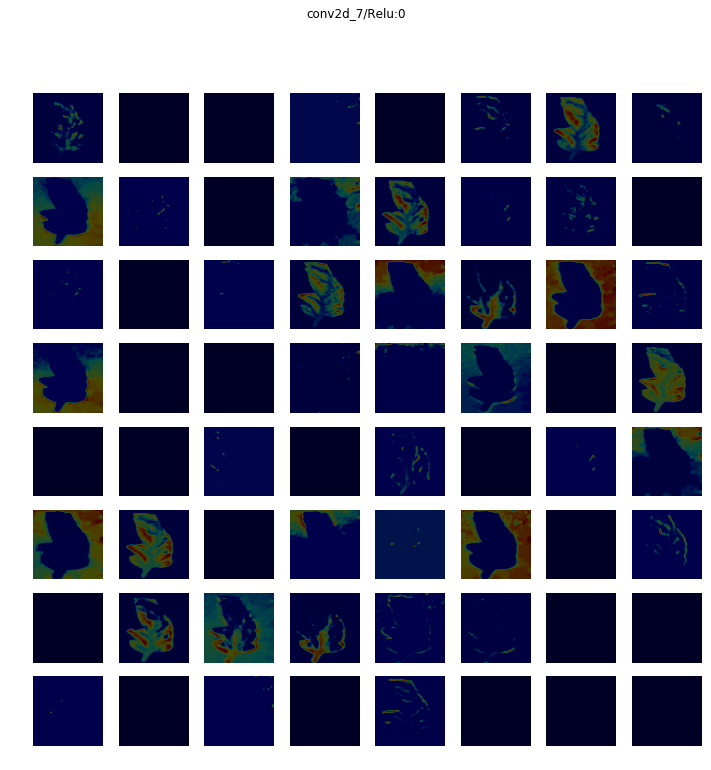
\includegraphics[width=\textwidth]{visualisierungen/yellow/heapmap_mit/conv2d_7.png}
	\caption{Visualisierung der Aktivierungswerte als Heatmap in der zweiten Faltungschicht von dem TYLCV-Virus (eigene Darstellung).}
	\label{}
\end{figure}

\begin{figure}[h!]
	\centering
	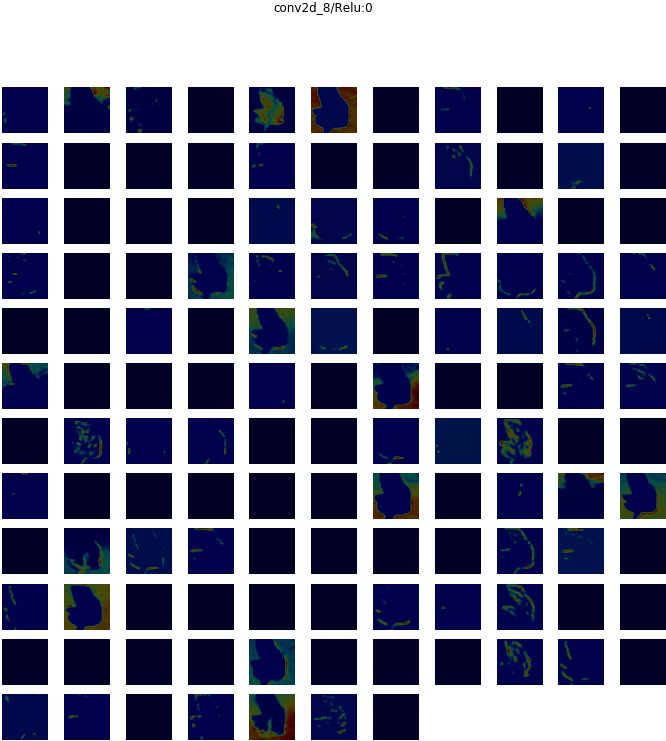
\includegraphics[width=\textwidth]{visualisierungen/yellow/heapmap_mit/conv2d_8.png}
	\caption{Visualisierung der Aktivierungswerte als Heatmap in der dritten Faltungschicht von dem TYLCV-Virus (eigene Darstellung).}
	\label{}
\end{figure}

\begin{figure}[h!]
	\centering
	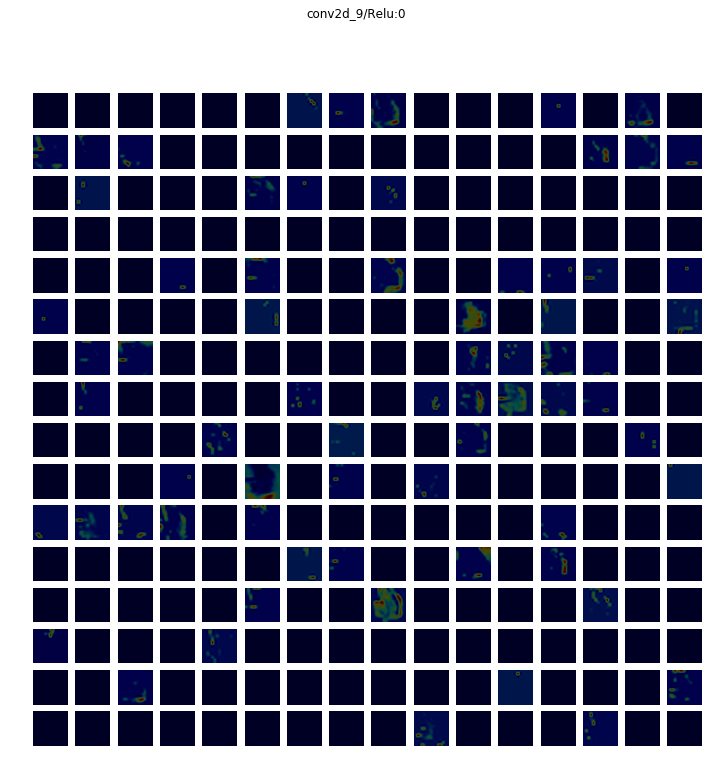
\includegraphics[width=\textwidth]{visualisierungen/yellow/heapmap_mit/conv2d_9.png}
	\caption{Visualisierung der Aktivierungswerte als Heatmap in der vierten Faltungschicht von dem TYLCV-Virus (eigene Darstellung).}
	\label{}
\end{figure}

\begin{figure}[h!]
	\centering
	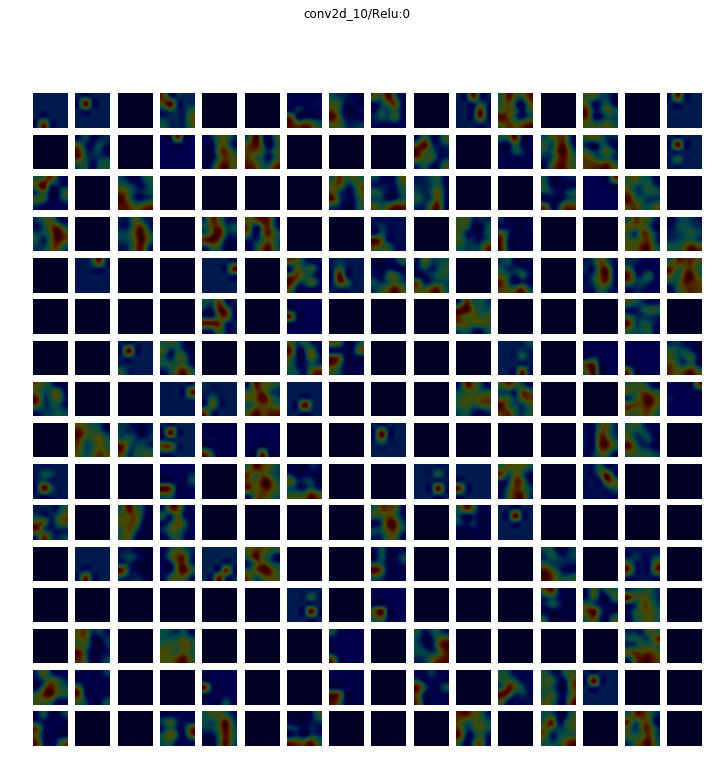
\includegraphics[width=\textwidth]{visualisierungen/yellow/heapmap_mit/conv2d_10.png}
	\caption{Visualisierung der Aktivierungswerte als Heatmap in der fünften Faltungschicht von dem TYLCV-Virus (eigene Darstellung).}
	\label{}
\end{figure}
